
	\section{GIS Module}

\subsection{Overview}
The GIS module provides services to gather, maintain, persist and provide information related to the world serviced by the system. It is about the creation and maintenance of a GIS Map of the
campus by using WiFi signal strengths and other available sources of GIS information. In addition it provides services to search for locations such as landmarks, buildings as well as venues such as offices, lecture halls and labs.

\subsection{External Interface Requirements}
This section gives a detailed description of the System Interfaces, hardware interfaces, software interfaces, communication interfaces and user interfaces.
\subsubsection{System Interfaces}
\begin{itemize}
\item The GIS module will interface with all subsystems or modules that work with location based data.

\item The GIS module will interface with the Navigation module in order to send and receive navigation information. The navigation module will send requests to the GIS module, these requests will include location information. The GIS module will use the location information to build map objects and the mapping unit in the GIS subsystem will plot the map objects on a map which is sent back to the Navigation module for use by the user.

\item The GIS module will interface with the Points of Interest module to create special gis objects like heritage sites and historic landmarks in the mapping subsystem of the GIS module

\end{itemize}


\subsubsection{User Interfaces}
The GIS subsystem will not directly interface with the user. All GIS related content will be shown to the user via the navigation subsystem.

\subsubsection{Hardware Interfaces}
The GIS module receives all its information from the navigation subsystem, thus it does not have any specific hardware interfaces.
\subsubsection{Software Interfaces}
\begin{itemize}
\item The GIS module will interface with the database in order to persist gis objects and retrieve location information needed to create gis objects.

\item The GIS module will use position tracking gps software such as \textbf{Position Logic} to track user movements and map the areas around them.
\end{itemize}

\subsubsection{Communication Interfaces}
The GIS subsystem does not communicate directly with the user, and it does not send out any notifications. Thus the GIS module has no communication interfaces.

\subsection{Performance Requirements}
The GIS module must be able to create a working area map that changes with the movements of the user. The map must be accurate within an area around the user to an extend that the user can view both large areas like buildings and smaller areas like offices. The generated map must be able to update or refresh at a rate high enough for it to be used effectively while walking on campus.

\subsection{Design Constraints}


The map produced by the GIS module should:
\begin{itemize}
\item be uncomplicated and convenient to use.

\item be straightforward and useful.

\item support viewing on all devices, taking into consideration different sized displays.

\item be colorized and visually appealing.

\item integrate easily with the navigation subsystem.

\item be user friendly to all target users, especially disabled users.

\item updated/refreshed efficiently so as to not annoy the user with lag or slow response times.
\end{itemize}
	
	\subsection{Software System Attributes} %

\subsubsection{Reliability}

The GIS module's primary purpose is to act as a database or a repository for all the map points in and around campus. For this reason it needs to meet the typical database standards of reliability, availability, scalability, and recoverability (RASR). The GIS module database should make be ACID compliant so that the typical CRUD operations of most databases can be performed as reliably as possible.

\subsubsection{Availability}

The GIS module should always be active as the majority of services the app provides are all dependant on the GIS module so to maintain the app's functionality it should have zero downtime. 



\subsubsection{Scalability}

The GIS module needs to be able to scale to handle a large amount of interactions so that it can still provide prompt feedback to users and not be slowed down or crash because of the large influx of user interaction.



\subsubsection{Recoverability}

The GIS module needs to be able to back up and recover the maps stored in it's database as well as all the map points stored on it so that system failures do not have catastrophic consequences.



\pagebreak

\subsection{UML}

\subsubsection{Class Diagram}

The GIS class diagram makes use of several design patterns. It makes use of Decorator for quick assembly of different types of objects that the map will use; it makes use of Strategy for different methods to search through the database; it makes use of Memento to back up and restore the map database; it makes use of Builder to separate the construction of complex map objects and their representation.



\begin{figure}[H]

	\centering

	\includegraphics[width=0.7\textwidth]{gis/Gis_class_diagram.png}

	\caption{GIS Class Diagram}

\end{figure}








\pagebreak

\subsubsection{Activity Diagram}

This diagram models work-flow activities of what users do when interacting with the GIS module.



\begin{figure}[H]

		\centering

		\includegraphics[width=\textwidth]{gis/GIS_Activity_Diagram.png}

		\caption{GIS Activity Diagram}

\end{figure}


\pagebreak


\subsubsection{Sequence Diagram}

This diagram models a user's interaction with the GIS module over time.

\begin{figure}[H]

		\centering

		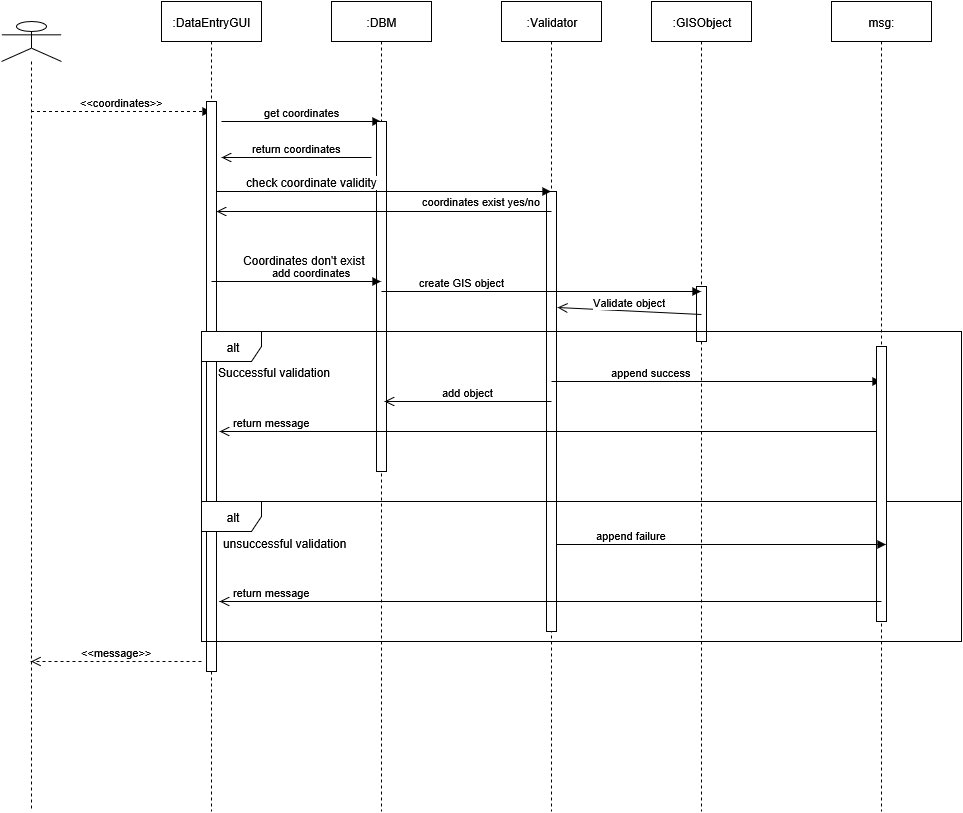
\includegraphics[width=0.7\textwidth]{gis/GIS_Sequence.jpg}

		\caption{GIS Sequence Diagram}

\end{figure}



\pagebreak



\subsubsection{State Diagram}

This diagram models state dependant behaviour of user interaction with the location-searching subsystem and the map-editing subsystem.

\begin{figure}[H]

		\centering

		\includegraphics[width=\textwidth]{gis/GIS_State_Diagram_final.png}

		\caption{GIS State Diagram}

\end{figure}





\pagebreak



\subsubsection{Use Case Diagram}

This is a use case diagram showcasing the interactions that users have with the GIS module

\begin{figure}[H]

		\centering

		\includegraphics[width=0.7\textwidth]{gis/GIS_use_case_diagram.png}

		\caption{GIS Use Case Diagram }

\end{figure}




